\subsection{Implementierung in Unity\hfill\textnormal{\emph{Berger}}}
Zusätzlich wurde der wurde Wechsel der Antriebe des Roboters 
noch einmal genauer in Unity implementiert.
Hierfür wurde das Modell aus Solidworks importiert 
und eine Beispiel Landschaft mit einem Wasser-Teich erstellt.
Für die Kamera wurde eine Skript geschrieben, 
dass dem Benutzer erlaubt die Kamera um den Roboter zu rotieren.

\subsection{Bewegung über Rigidbodys} \label{sec:rigidbody_switch}
Die Bewegung des Roboters ist mit der Physik-Simulation von Unity realisiert.
Dabei gibt es sogenannte "Rigidbodys", die einem Objekt zugewiesen werden können
und Kollision und Gravitation umsetzen.
Zusätzlich ist es möglich beliebige Kräfte auf die Rigidbodys einwirken zu lassen.
Unser Rescue-Robot besteht in Unity aus einem Rigidbody für das Chassis,
jeweils einem für jede Kette
und einem für den Propeller.
Sie sind mit sog. "fixed-joints" verbunden 
und sind wie in Abbildung \ref{fig:unity1} dargestellt positioniert.
Dort sind zu Veranschaulichung farbige Sphären um den Schwerpunkt und 
Kraft-Ansatzpunkt der Rigidbodys gezeichnet.


\begin{figure}[H]
  \centering{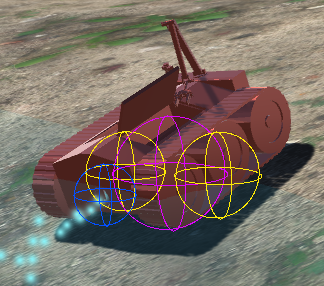
\includegraphics[width=0.8\linewidth]{Abbildungen/unity1.png}}
  \caption{Roboter in Unity}
  \label{fig:unity1}
\end{figure}

Solange der Roboter Kontakt mit festem Untergrund erkennt, 
läuft die Fortbewegung über die Rigidbodys der Ketten.
In diesem Modus kann der Roboter sich entweder geradeaus nach vorne und hinten bewegen, 
oder sich auf der Stelle drehen.
Dies wird manuell vom Benutzter über die WASD-Tasten auf der Tastatur gesteuert.
Die gewählte Richtung wird mit der Variable für die Kraft der Ketten multipliziert 
und als Kraft auf die Ketten angebracht.
Da die Rigidbodys mit den fixed-joints verbunden sind, 
wird dadurch der gesamte Roboter bewegt.(NFR1)

Falls der Roboter Wasser berührt, läuft die Kraft stattdessen durch den Propeller.(FR7)
Dabei wird ihm zusätzlich die Funktion des Ruders gegeben,
das heißt falls zu Seite gesteuert wird,
wirkt ein Drehmoment auf den Propeller und somit auf den gesamten Roboter.(NFR2)

Das schwimmen auf dem Wasser wurde deutlich vereinfacht umgesetzt.
Ein halb transparenter Quader stellt das Wasser visuell dar
und eine unsichtbare Ebene knapp unter der Oberfläche 
sorgt für die Kollision mit dem Roboter.

\subsection{Tests mit autonomen Fahren}
Separat wurde das Skript \texttt{autoDrive.cs} erstellt. 
Dieses richtet den Roboter auf ein vorher zugewiesenes Objekt aus 
und lässt ihn in diese Richtung fahren.
Beides findet auch hier physikalisch korrekt über Rigidbodys 
und einer festgelegten Motorkraft statt.
Der Roboter überschießt dabei sowohl bei drehen als auch beim fahren sein Ziel nicht, 
sondern nähert sich erst immer schneller und immer langsamer an.
Dieses Skript benutzt allerdings nicht den komplexeren Rigidbody-Aufbau 
aus Abschnitt \ref{sec:rigidbody_switch}, 
sondern wirkt alle Kräfte direkt auf den Haupt-Körper.